\newcommand{\mess}[3] {
\begin{figure}[htbp]
	\centering
	\includegraphics[width=0.8\textwidth]{#1}
	\caption{#2}
	\label{#3}
\end{figure} }
\newcommand{\refabb}[1]{(siehe Abb. \ref{#1})}
\chapter{Durchführung}

\section{Solarzelle}
Als Solarzelle kommt eine Anordnung von 6 Einzelzellen zum Einsatz. Zuerst messen wir die Leerlauf und den Kurzschlussstrom der Anlage bei verschiedenen Beleuchtungsstärken.
\begin{center}
\begin{tabular}{ |  l  c  c  c | }
\hline
	& Tisch	& Fenster & unter Tisch \\ \hline	
Leerlaufspannung & $\SI{0,665}{\volt}$	& $\SI{1,979}{\volt}$	& $\SI{0,173}{\volt}$ \\ 
Kurzschlussstrom & $\SI{0,95}{\milli \ampere}$	& $\SI{9,89}{\milli \ampere}$	& $\SI{0,18}{\milli \ampere}$ \\ 
\hline
\end{tabular}
\end{center}

Wir messen nun die I/U-Kennlinie der Zellen im Dunklen \refabb{a2}.
Aus dieser Kennlinie erzeugen wir die P/I-Kennlinie. Im Dunklen ist die Leistung hier positiv, die Zellen wirken also als Verbraucher \refabb{a2pi}. 
\mess{mess/aufg2.pdf}{Dunkel I/U-Kennlinie der Solarzellen}{a2}
\mess{mess/aufg2_pi.pdf}{Dunkel P/I-Kennlinie der Solarzellen: Zellen wirken als Verbraucher}{a2pi}

Nun messen wir die I/U-Kennlinie bei beleuchteter Zelle. Dazu schalten wir verschiedene Lastwiderstände vor \refabb{a3}. 
\mess{mess/aufg3_iu.pdf}{I/U-Kennlinie der Solarzellen}{a3}
Aus dieser erzeugen wir wiederum die P/I-Kennlinie \refabb{a3pi}
\mess{mess/aufg3_pi.pdf}{P/I-Kennlinie der Solarzellen}{a3pi} 
Gefittet wurde die I/U-Kennlinie mit dem Zusammenhang:
\[
I(U) = y_0 + I_0 \, e^{\frac{U}{U_0}}
\]
Aus dem Fit ergeben sich die Werte:
\begin{align*}
	y_0 &= \SI{-9.48}{\milli \ampere}\\
	I_O &= \SI{0.28}{\milli \ampere}\\
	U_0 &= \SI{0.55}{\volt}
\end{align*}

Verunreinigungen und Kristallfehler and der Grenzfläche der p-n leitenden Schicht verursachen Widerstände die sich im realen nicht auf 0 (Reihe) und unendlich (Parallel) setzen lassen.
Dabei wäre der Füllfaktor bei 1 und der MPP folglich am besten.
Um diese Widerstände zu bestimmen nutzt man die Kennlinie des Bauteils.
Diese Widerstände entsprechen den Steigungen der Kennlinie nahe den Achsen, also der Steigung des Graphen bei Leerlaufspannung und Kurzschlussstrom.
Wir erhalten daraus die Werte:
\[
R_p=\SI{38}{\kilo \joule} \quad
R_S=\SI{746}{\ohm}
\]
Diese Werte sind in etwa realistisch für unsere Bedingungen. Die Tendenz, dass der Parallelwiderstand hoch ist und der Reihenwiderstand gering ist, ist gegeben. Die Werte wurden am Fenster aufgenommen.

\section{Brennstoffzelle}
Zunächst gilt es wiederum die I/U-Kennlinie aufzuzeichnen. Hierfür variieren wir die Elektrolyseurspannung und messen den zugehörigen Strom.
\begin{figure}[htbp]
	\centering
	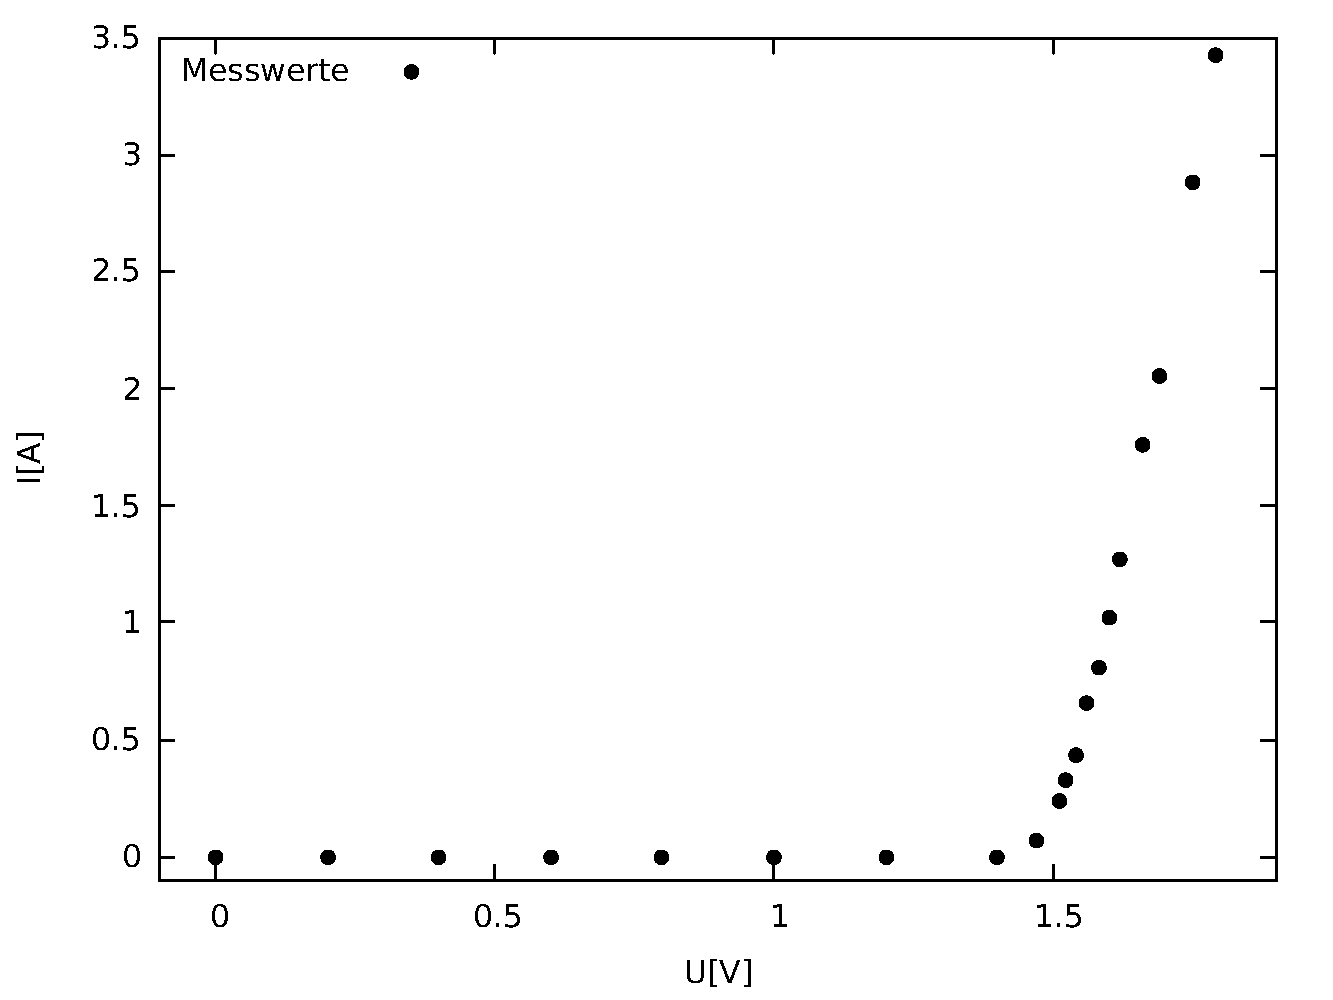
\includegraphics[width=0.8\textwidth]{mess/aufg7.pdf}
	\caption{I/U-Kennlinie des Elektrolyseurs: Nach dem Erreichen der Zersetzungsspannung von ca. 1,5 Volt, nimmt der Strom linear zu}
	\label{a7}
\end{figure}

Nun wollen wir den elektrischen Wirkungsgrad des Elektrolyseur bestimmen. Hierfür benötigen wir den Brennwert für Wasserstoff. 
Die geleistete Arbeit des Elektrolyseurs ist proportional zum erzeugen Gasvolumen V. Mit der Formel $W_{el}=UIt$ kann man nun die theoretisch mögliche Spannung berechnen und damit den elektrischen Wirkungsgrad bestimmen.
\begin{figure}[htbp]
	\centering
	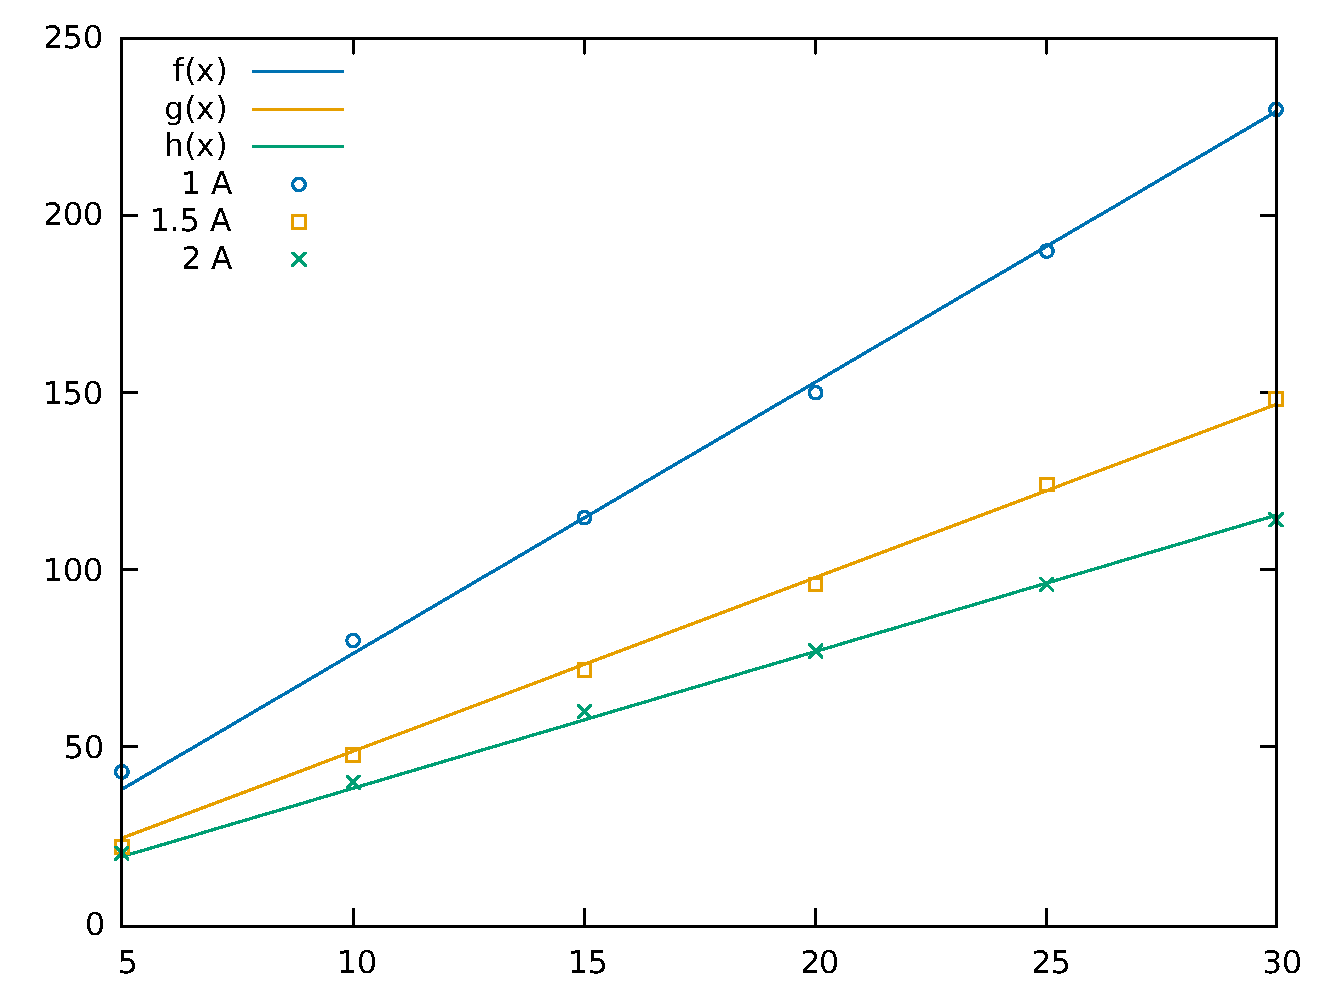
\includegraphics[width=0.8\textwidth]{mess/aufg8.pdf}
	\caption{lol keine Ahnung mann}
	\label{a8}
\end{figure}

\[ n=\frac{W_{HV}}{W_{el}} \]
\[
n(\SI{1}{\ampere})=0,95 \quad
n(\SI{2}{\ampere})=0,96 \quad
n(\SI{2,5}{\ampere})=0,92
\]
Diese Werte sind sehr gut. Eine gute Ausbeute bei der Aufspaltung von $H_2O$ ist wünschenswert. Dies zeigt, dass die Herstellung von Wasserstoff sehr effizient ist. Mit dem Gas betreibt man später eine Brennstoffzelle.

Im Folgenden berechnen wir das Verhältnis von theoretisch errechneter zu tatsächlich erzeugter Gasmenge. Dadurch lässt sich die Beziehung zum Faraday’schen Gesetz überprüfen. Nutzt man die Formeln:
$Q=nzF$
mit dem molaren Volumen $V_m=V_n=\SI{24,465}{\litre}$,
z=2 (es werden beide H-Atome des $H_2O$ reduziert)
$I=\frac{VzF}{Vnt}$
$\frac{dV}{dt}=I \cdot \SI{0.127}{\centi \meter \cubed \per \ampere \second}$
Berechnen sich unsere Faraday’schen Widerstände auf:
\[
nF(1A)=1,02 \quad nF(2A) = 1,05 \quad nF(2,5A)=1,04
\]
Die Werte sind größer als eins, was auf manche Fehlerquellen verweisen muss. Da dieses Gesetz die chemischen Vorgänge beschreibt, sollte die Werte auch nahe an der eins liegen. Probleme stellten beispielsweise das Ablesen der Gasmenge dar. Die angebrachte Skala war recht unhandlich und grob abzulesen.

Auch für die Brennstoffzolle soll nun die I/U-Kennlinie aufgenommen werden. Hierzu wird der zwischengeschaltete Widerstand variiert.
\begin{figure}
	\centering
	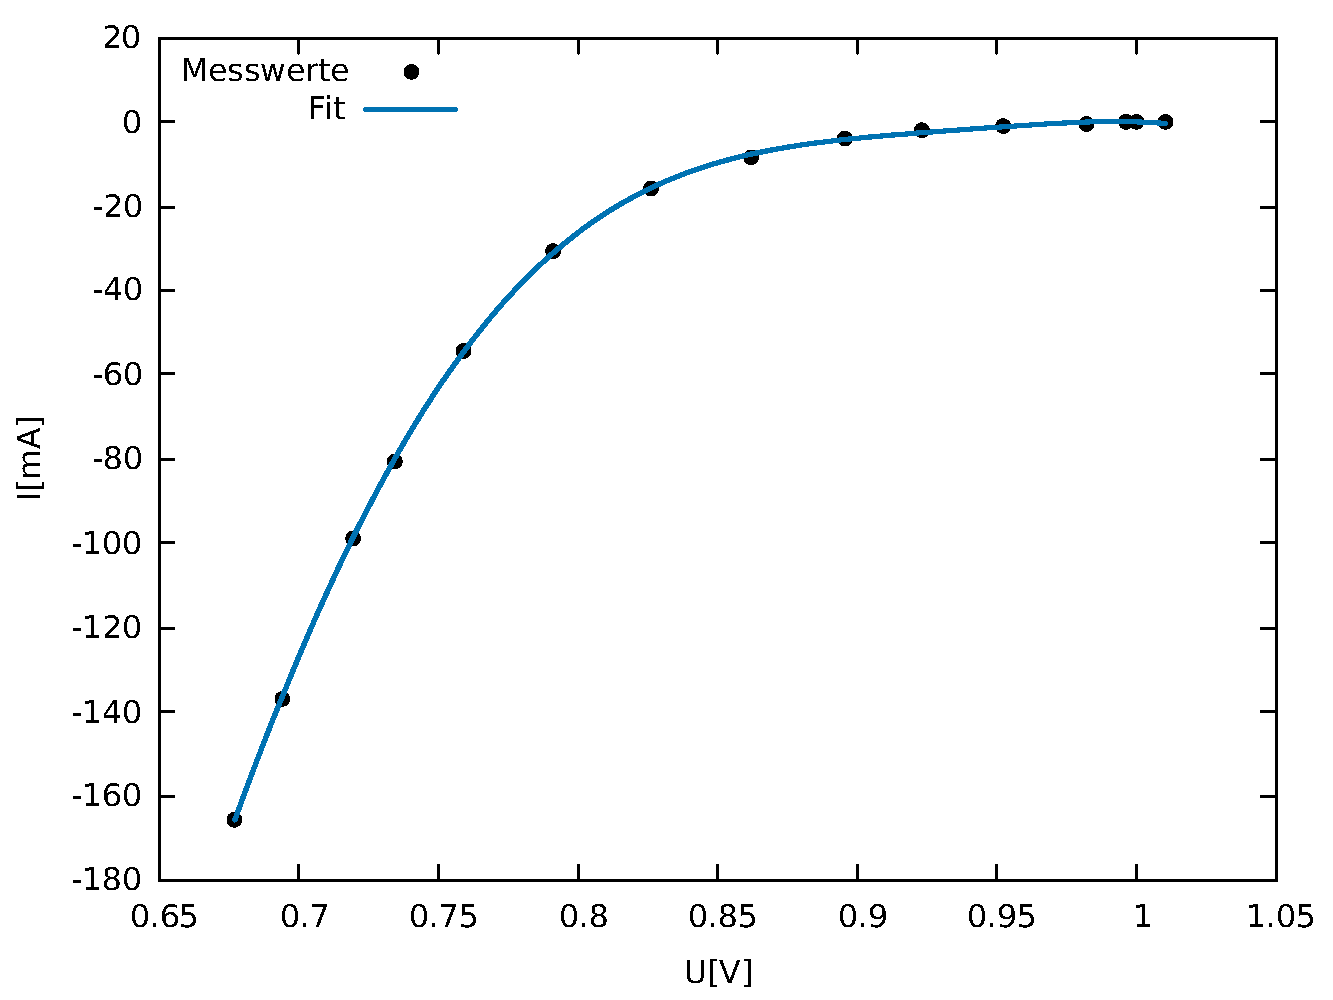
\includegraphics[width=0.8\textwidth]{mess/aufg10.pdf}
	\caption{I/U-Kennlinie der Brennstoffzelle: durch den, auch ohne zusätzlich vorgeschaltetes Bauteil, hohen Widerstand des Aufbaus, ist die Kennlinie linear}
	\label{a10}
\end{figure}

Nun soll der Maximum Power Point bestimmt werden. Hierzu nutzen wir die P/I Kennlinie und erkennen, dass unsere P/I Kurve bis zum Ende hin steigt. Wir konnten keinen geringeren Widerstand als $\SI{0,8}{\ohm}$  in den Stromkreis einschließen und der Kurzschlussstrom kann die Brennstoffzelle zerstören. Wir benennen also unseren MPP an der Stelle von 0,8 Ohm und bekommen folgenden Wert: PMPP = 95mW 
Dieser Wert ist akzeptabel.
\begin{figure}[htbp]
	\centering
	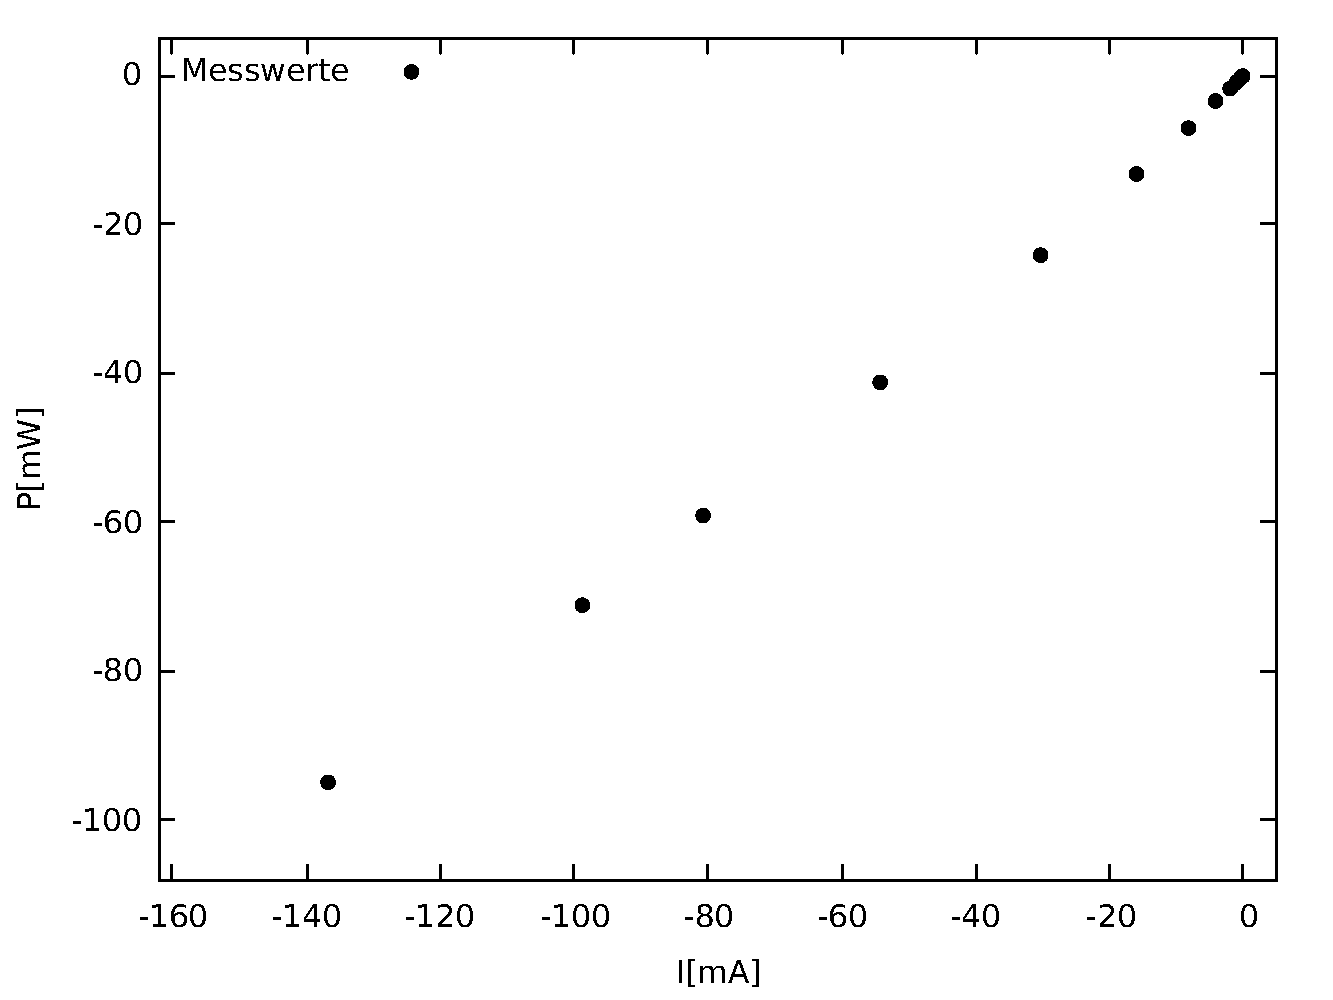
\includegraphics[width=0.8\textwidth]{mess/aufg11.pdf}
	\caption{P/I-Kennlinie der Brenstoffzelle: linearer Anstieg}
	\label{a11}
\end{figure}

Nun soll bei konstanter Last die verbrauchte Gasmenge bestimmt werden:
\begin{figure}[htbp]
	\centering
	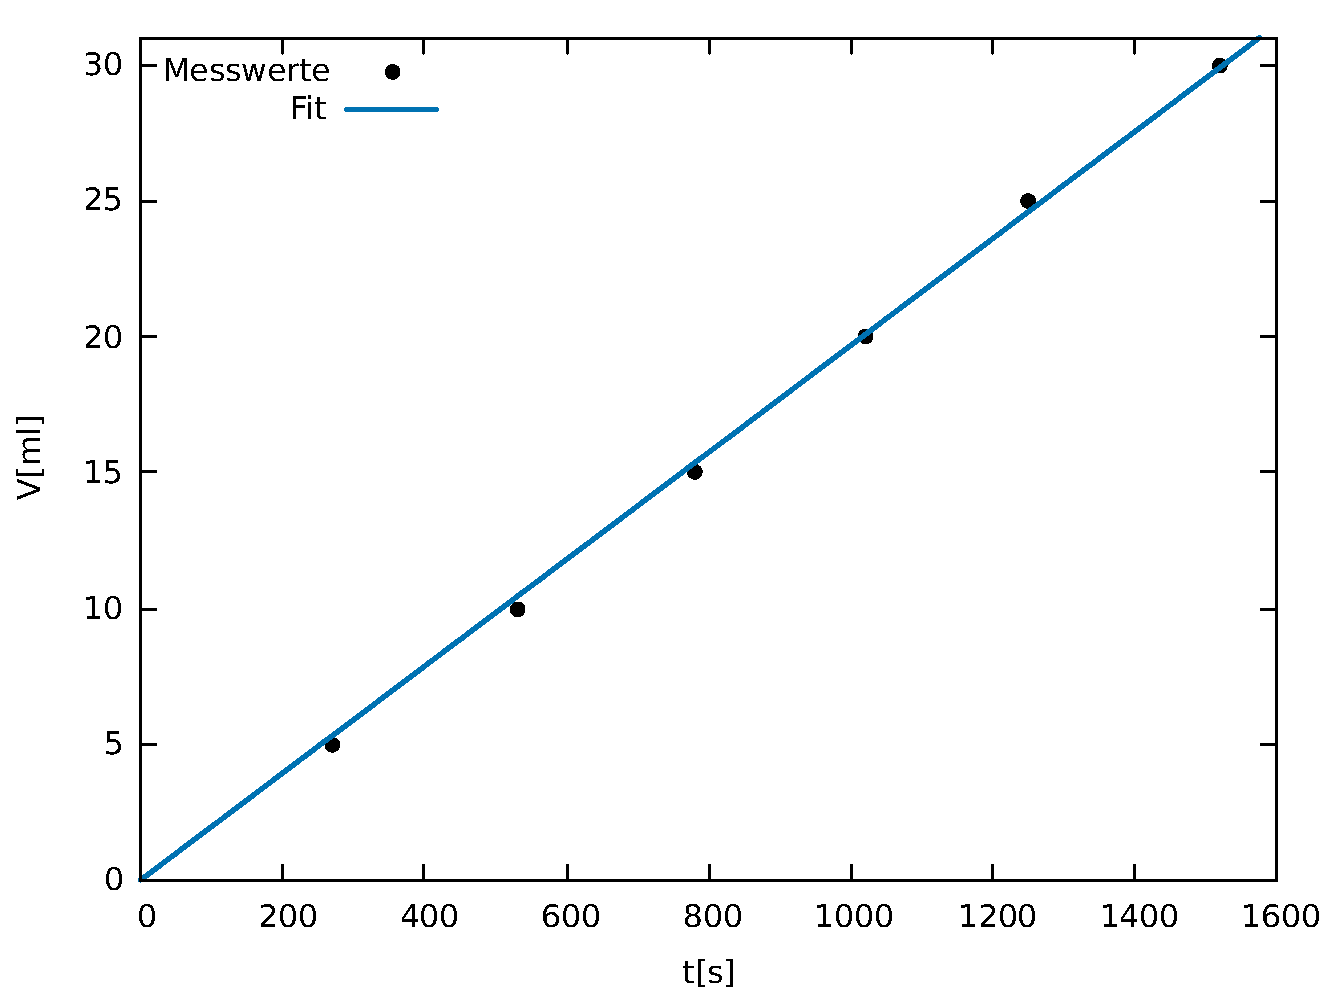
\includegraphics[width=0.8\textwidth]{mess/aufg12.pdf}
	\caption{Gasmenge pro Zeit, Last an Brennstoffzelle konstant}
	\label{a12}
\end{figure}
Wir bestimmen nun analog zum Elektrolyseur den elektrischen und Faraday’schen Wirkungsgrad der Brennstoffzelle.
Bei $\SI{0.13}{\volt}$ und $\SI{-128}{\milli \ampere}$ hat die Zelle am meisten Gas verbraucht uns somit am meisten Leistung gebracht. Für uns Ergeben sich folgende Werte:
\begin{align*}
n_el &= \frac{W_{el}}{HHH2V}=0,39
n_F &= \frac{V_{theo}}{V}=0,83
\end{align*}
Klar war für uns, die Erzeugung von Strom durch den Verbrauch von Wasserstoff und Sauerstoff zu Wasser kann nicht perfekt Funktionieren. Dennoch ist sie mit ca. 40\% besser als die meisten Stromerzeuger. Theoretisch sind wohl auch noch bessere Werte möglich, mit geringerem Widerstand und einer moderneren Vorrichtung.
